\documentclass[11pt]{article}
% Shared preamble for Group 3 reports. Compile from each paper's directory
% with pdflatex + bibtex (see compile.ps1).
\usepackage[a4paper,margin=2.2cm]{geometry}
\usepackage[T1]{fontenc}
\usepackage[utf8]{inputenc}
\usepackage{lmodern}
\usepackage{microtype}
\usepackage{setspace}
\usepackage{booktabs}
\usepackage{tabularx}
\usepackage{longtable}
\usepackage{array}
\usepackage{graphicx}
\usepackage{tikz}
\usetikzlibrary{arrows.meta,positioning,shapes.geometric}
\usepackage{hyperref}
\usepackage{xcolor}
\usepackage[authoryear,round,sort]{natbib}
\usepackage{titlesec}
\usepackage{enumitem}
\usepackage{caption}
\usepackage{fancyhdr}

\onehalfspacing
\setlist[itemize]{leftmargin=1.4em,itemsep=0.25em}
\setlist[enumerate]{leftmargin=1.4em,itemsep=0.25em}
\hypersetup{colorlinks=true,linkcolor=black,citecolor=black,urlcolor=blue}

\newcommand{\groupcover}[1]{%
  \begin{center}
    
\includegraphics[width=2.6cm]{../uct_logo.jpg}\\[0.7em]
    {\large University of Cape Town}\\[0.4em]
    {\large ECO5040W --- Financial Software Engineering}\\[1.2em]
    {\LARGE\bfseries #1}\\[1.0em]
    {\large XRPL-Based FX Remittance Platform using RLUSD}\\[1.4em]
    Annita Ngoma \quad Karabo Tigedi \quad Kerry-Lynn Whyte\\[0.35em]
    Liltha Mzamo \quad Nikola Milosavljevic\\[0.3em]
    {\small Group 3}\\[0.6em]
    {\small 7 September 2026}
  \end{center}
  \vspace{1.2em}
}

\usepackage{amsmath}
\usepackage{float}

\begin{document}
\emergencystretch=3em
\groupcover{Business and Technical Specification}

\noindent
This specification describes \textbf{Group 3's} XRPL remittance prototype as implemented in this GitHub fork (Karabo22Tigedi / FSE-Project). An earlier GitHub sketch by Kerry-Lynn Whyte established FastAPI, SQLite, Redis Streams, and Testnet Payments. This document is about \emph{our} patched system, not that sketch. Cash-in and cash-out remain simulated. Using a dollar stablecoin does not remove South African exchange-control, anti-money-laundering, or licensing duties \citep{UCTBrief2026}. One hundred and twenty-nine automated tests currently pass. The examiner-facing product is the Vite React UI in \texttt{frontend/} (Section~\ref{sec:ui}), talking to FastAPI on port 8000.

\section{Business problem}
Cross-border remittances move household income to people who often collect cash at an agent. Western Union and MoneyGram are the familiar brands: the sender pays rand at an agent or online, the operator takes a fee, and the recipient collects cash on the other side after showing identification. Those operators are large, licensed money transmitters with agent networks in many countries. They are also expensive on small sends, and the price the customer sees is often a mix of a posted fee and a worse-than-mid-market exchange rate.

The World Bank's Remittance Prices Worldwide (RPW) survey is the standard public comparison of corridor costs \citep{WorldBankRPW}. South Africa is a high-cost sending market on that survey. Rateweb's 2026 reading of the 2025~Q1 RPW release reports Western Union and MoneyGram flat fees of about R214--R217 on a surveyed send of about R1{,}370 \citep{Rateweb2026}. That is a fee of roughly 15--16\% of the send amount before any FX spread. For a family sending grocery money, that is a large bite.

Cost is not the only friction. The IMF's diagnostic of the South Africa--Zimbabwe corridor describes cash-heavy, agent-based payouts, delays, and weak price transparency \citep{IMF2025SAZim}. FinMark Trust's 2024 assessment of South Africa to the rest of SADC likewise finds that cash collection and agent processes still dominate, and that customers often cannot see the full cost until they are already at the counter \citep{FinMark2024}. Western Union and MoneyGram solve a real problem---getting cash to someone without a bank account---but they do it with many intermediaries, posted-plus-spread pricing, and a payout model that is slow to digitise.

Stablecoins such as RLUSD (a US-dollar token issued on the XRP Ledger) can move value between wallets in seconds once both sides hold the token. That does not magically replace the cash-in door in Johannesburg or the cash-out door in Harare. The brief is explicit: a prototype may \emph{simulate} those fiat legs \citep{UCTBrief2026}. Our platform therefore uses UCTUSD (Marc's course IOU) as the current \emph{settlement} asset between a confirmed rand payment and a custodial recipient wallet; the API slot remains \texttt{rlusd\_amount} and can later point at official RLUSD via \texttt{.env} if funded. We do not claim that putting value on a ledger deletes the South African Reserve Bank, FICA, or a remittance licence.

What we do claim, as a design, is narrower. A quoted fee of a fixed rand amount plus a percentage, plus a published FX margin on the conversion rate, is easier to audit than an opaque corridor tariff. A 15-minute quote with an explicit cancel path stops abandoned drafts from consuming a sender's daily limit. An on-chain Payment with a stored transaction hash gives the recipient something they can look up on a Testnet explorer. Those are the product bets this specification implements.

\section{User journey}
The journey follows the brief \citep{UCTBrief2026} and is implemented end-to-end on the API and on the web UI in Section~\ref{sec:ui}.

\begin{enumerate}
  \item A customer registers (\texttt{POST /auth/register}) and logs in (\texttt{POST /auth/login}). The same customer account can send or receive; role is \texttt{customer} or \texttt{admin}, not two person types.
  \item The sender submits mock KYC (\texttt{POST /kyc}). An admin approves or rejects it. Unapproved senders cannot create quotes.
  \item The sender adds a beneficiary (\texttt{POST /beneficiaries}). If mobile or email already matches a registered user, the record links immediately; if the recipient registers later, linking happens then.
  \item The sender posts a ZAR amount (\texttt{POST /remittances}). The API fetches USD/ZAR, applies the fee model, checks daily and monthly limits, and returns a quote with \texttt{tracking\_ref} (\texttt{MG} plus ten digits) and \texttt{expires\_at} (15 minutes).
  \item The sender may cancel an unexpired quote (\texttt{POST /remittances/\{id\}/cancel}) or let it expire. Cancelled and expired quotes do not consume limits.
  \item The sender initiates simulated cash-in (agent cash, bank transfer, or card). An admin confirms receipt. Settlement is not queued before that confirmation.
  \item A Redis Streams worker submits an XRPL Testnet Payment from the platform treasury to the recipient's custodial account, stores the hash, and credits the internal spendable balance.
  \item The recipient opens \texttt{GET /wallet/me}, sees spendable UCTUSD, incoming transfers with hashes, and cash-out history.
  \item The recipient requests a cash-out to USD or ZAR. Fiat payout is still simulated, but complete submits a Payment of the reserved UCTUSD from the recipient custodial account to the official UCTUSD issuer (burn/redeem). \texttt{on\_chain\_balance} excludes completed cash-outs. Failed cash-outs refund spendable balance.
\end{enumerate}

Anyone with a tracking reference who is the sender, the linked recipient, or an admin can open \texttt{/app/track/\{ref\}} or call \texttt{GET /remittances/track/\{ref\}}.

\section{Functional requirements}
Table~\ref{tab:fr} maps the brief's required behaviour to \emph{our} endpoints. Interactive OpenAPI lives at \texttt{/docs}. \texttt{GET /health} is unauthenticated.

\begin{table}[ht]
\centering
\caption{Functional behaviour mapped to this fork's API.}
\label{tab:fr}
\footnotesize
\begin{tabular}{@{}p{0.28\textwidth}p{0.66\textwidth}@{}}
\toprule
\textbf{Capability} & \textbf{Our implementation} \\
\midrule
Register, login, logout, profile &
\texttt{POST /auth/register}, \texttt{/auth/login}, \texttt{/auth/logout};
\texttt{GET}/\texttt{PATCH /users/me}. Passwords bcrypt; sessions hashed at rest. \\
Mock KYC + admin review &
\texttt{POST /kyc}; \texttt{GET /kyc/me}, \texttt{/kyc/me/status};
admin \texttt{GET /kyc}, \texttt{POST /kyc/\{id\}/approve\textbar reject}.
ID number encrypted with the KYC Fernet key. \\
Beneficiaries &
\texttt{POST}/\texttt{GET /beneficiaries}. Auto-link on mobile/email. \\
Quote, fees, limits &
\texttt{POST /remittances}; \texttt{GET /limits/me};
admin \texttt{GET}/\texttt{PUT /admin/fee-config},
\texttt{GET}/\texttt{PUT /admin/limit-tiers/\{tier\}}. \\
Quote lifecycle &
TTL 15 minutes; \texttt{POST /remittances/\{id\}/cancel};
cash-in rejected if expired or cancelled;
fee-consumes-send rejected with 422. \\
Tracking &
\texttt{tracking\_ref} on \texttt{RemittanceOut};
\texttt{GET /remittances/track/\{ref\}}. \\
Simulated cash-in &
\texttt{POST /remittances/\{id\}/cash-in};
admin \texttt{POST \ldots/confirm-cash-in} enqueues settlement. \\
Queued XRPL settlement &
Redis Stream \texttt{settlement\_messages};
\texttt{POST /admin/settlement/run};
\texttt{GET /admin/settlement};
\texttt{POST /admin/settlement/\{id\}/retry}
(pending, processing, or failed; completed is 409). \\
Custodial wallet &
\texttt{GET /wallet/me}: \texttt{balance\_rlusd} = spendable;
also \texttt{spendable\_balance} and \texttt{on\_chain\_balance}
(excludes completed cash-outs).
Admin \texttt{GET /admin/platform-wallet} reports treasury address,
TrustLine, and UCTUSD liquidity. \\
Simulated cash-out &
\texttt{POST /cash-outs}; \texttt{GET /cash-outs/me};
admin list/approve/complete/fail. USD and ZAR only. \\
Sender history &
\texttt{GET /remittances/me}; admin \texttt{GET /remittances}. \\
\bottomrule
\end{tabular}
\end{table}

\section{Fee model}
Fees are a single admin-editable \texttt{FeeConfig} row, not a history table. Percentages are fractions (0.0100 means 1\%). Seeded defaults are a R25.00 fixed fee, 1\% of send, 2\% FX margin, and 1.5\% cash-out.

Let \texttt{zar} be the send amount, \texttt{fixed} and \texttt{percentage} the transaction-fee parameters, \texttt{midmarket} the USD/ZAR rate, and \texttt{fx\_margin} the spread fraction. Then:
\begin{align*}
\texttt{transaction\_fee} &= \texttt{fixed} + \texttt{zar}\times\texttt{percentage} \\
\texttt{effective\_rate} &= \texttt{midmarket}\times(1+\texttt{fx\_margin}) \\
\texttt{net\_zar} &= \texttt{zar} - \texttt{transaction\_fee} \\
\texttt{rlusd} &= \texttt{net\_zar}\,/\,\texttt{effective\_rate}
\end{align*}
The quote is rejected (HTTP 422) if \texttt{rlusd} $\le 0$ (equivalently if net ZAR after the transaction fee is not positive). Transaction fees are rounded to two decimal places; RLUSD amounts to six, half-up. RLUSD is treated as 1:1 with USD.

The FX margin makes the sender's conversion \emph{worse} than mid-market: more rand per dollar means fewer dollars received. The cash-out percentage shown on the remittance quote is an \emph{estimate}. At cash-out time the fee is reapplied to the RLUSD amount, USD is 1:1 after that fee, and ZAR cash-out uses the live (or fallback) USD/ZAR rate \emph{without} the FX margin.

\subsection{Worked example}
Using seeded defaults and the configured fallback mid-market rate of 18.50 (the live API may differ; the algebra does not). For a R1{,}370.00 send, comparable to the RPW send size discussed by \citet{Rateweb2026}:
\begin{align*}
\texttt{transaction\_fee} &= 25.00 + 1370.00\times 0.01 = 38.70 \\
\texttt{effective\_rate} &= 18.50\times 1.02 = 18.87 \\
\texttt{net\_zar} &= 1370.00 - 38.70 = 1331.30 \\
\texttt{rlusd} &= 1331.30 / 18.87 = 70.551139
\end{align*}
Estimated cash-out fee $= 70.551139 \times 0.015 = 1.058267$ RLUSD; estimated recipient payout $= 69.492872$ RLUSD. The transaction fee (R38.70) is far below the R214--R217 Western Union / MoneyGram flat fees on that send size \citep{Rateweb2026}. That comparison is indicative only: our cash legs are simulated, we are not an agent network, and a live mid-market rate plus a 2\% margin is not a licensed tariff.

A send whose fee consumes the principal is rejected. At the same defaults, R25.00 yields a R25.25 fee and a negative net, so the API returns 422.

Table~\ref{tab:fees} is the seeded \texttt{FeeConfig} an admin can edit at \texttt{PUT /admin/fee-config}. There is no fee-history table: the live row is what the next quote uses.

\begin{table}[ht]
\centering
\caption{Seeded fee parameters (fractions, not whole percents).}
\label{tab:fees}
\begin{tabular}{@{}llr@{}}
\toprule
\textbf{Field} & \textbf{Meaning} & \textbf{Default} \\
\midrule
\texttt{fixed\_fee\_zar} & Rand added to every send & 25.00 \\
\texttt{percentage\_fee} & Share of send ZAR & 0.0100 \\
\texttt{fx\_margin\_percentage} & Added to mid-market rate & 0.0200 \\
\texttt{cash\_out\_fee\_percentage} & Share of RLUSD at cash-out & 0.0150 \\
\bottomrule
\end{tabular}
\end{table}

\section{Exchange rates}
The brief allows a public API, a mock service, or a configured table \citep{UCTBrief2026}. We use the first, with the third as fallback. \texttt{GET https://open.er-api.com/v6/latest/USD} supplies \texttt{rates.ZAR}. Successes are cached for 300 seconds (\texttt{EXCHANGE\_RATE\_CACHE\_SECONDS}) so concurrent quotes do not stampede a free endpoint. Any failure (network, timeout, non-2xx, missing ZAR field) uses \texttt{USD\_ZAR\_RATE} from \texttt{.env} (default 18.50). There is no admin API for the fallback; changing it means editing the environment and restarting, and it only matters while the live API is down. Tests mock the live call except for dedicated exchange-rate tests.

\section{Remittance limits}
Tiers are derived from KYC, not stored on the user: approved $\to$ \texttt{verified}, otherwise \texttt{unverified}. Seeded caps match the brief's example: unverified R0 / R0 per day and month; verified R3{,}000 / R25{,}000. Admins may change caps via \texttt{PUT /admin/limit-tiers/\{tier\_key\}}. Unverified is not reachable through \texttt{POST /remittances} because that route requires approved KYC; the zero caps still exist so the example table is configurable.

Usage sums the sender's ZAR since the start of the UTC day or calendar month, with two exclusions that the original sketch did not have: \texttt{cancelled} never counts; \texttt{quoted} rows with \texttt{expires\_at} already in the past never count. Unexpired quotes and every later live status---including \texttt{settlement\_failed}---do count. That is deliberate: a failed on-chain payment still represents a confirmed cash-in that occupied limit capacity until an operator decides otherwise.

\begin{table}[ht]
\centering
\caption{Remittance statuses on one evolving row.}
\label{tab:status}
\footnotesize
\begin{tabular}{@{}lll@{}}
\toprule
\textbf{Status} & \textbf{How we get there} & \textbf{Counts to limit?} \\
\midrule
\texttt{quoted} & \texttt{POST /remittances} & Yes, until TTL \\
\texttt{cancelled} & sender cancel, still unexpired & No \\
\texttt{quoted} past TTL & clock; cash-in 409 & No \\
\texttt{cash\_in\_pending} & sender cash-in & Yes \\
\texttt{cash\_in\_confirmed} & admin confirm & Yes \\
\texttt{settlement\_queued} & enqueue after confirm & Yes \\
\texttt{settled} & worker Payment + credit & Yes \\
\texttt{settlement\_failed} & worker error; no credit & Yes \\
\bottomrule
\end{tabular}
\end{table}

\section{Architecture}
\label{sec:arch}
Figure~\ref{fig:arch} is the runtime. The Vite React app on 5173 (or 5174 if 5173 is busy) is the marked web UI. FastAPI serves JSON. SQLAlchemy talks to SQLite through Alembic revisions \texttt{0001\_initial}, \texttt{0002\_quote\_session}, and \texttt{0003\_cash\_out\_burn}. Redis is transport for settlement, not the source of truth. The settlement worker (the same function as \texttt{POST /admin/settlement/run} and \texttt{python -m scripts.run\_settlement\_worker}) signs Testnet Payments with \texttt{xrpl-py}. CORS allows the local Vite and API origins, including loopback.

\begin{figure}[ht]
\centering
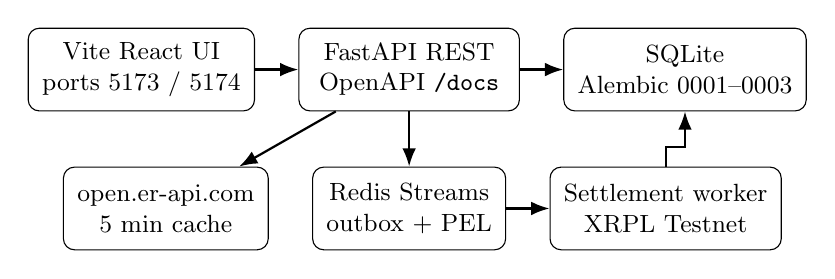
\begin{tikzpicture}[
  font=\small,
  box/.style={draw, rounded corners, align=center, inner sep=5pt, minimum height=1.05cm},
  arr/.style={-{Latex}, thick}
]
\node[box, minimum width=2.6cm] (ui) {Vite React UI\\ports 5173 / 5174};
\node[box, minimum width=2.8cm, right=0.55cm of ui] (api) {FastAPI REST\\OpenAPI \texttt{/docs}};
\node[box, minimum width=2.4cm, right=0.55cm of api] (db) {SQLite\\Alembic 0001--0003};
\node[box, minimum width=2.3cm, below=0.7cm of api] (redis) {Redis Streams\\outbox + PEL};
\node[box, minimum width=2.6cm, left=0.55cm of redis] (fx) {open.er-api.com\\5 min cache};
\node[box, minimum width=2.6cm, right=0.55cm of redis] (worker) {Settlement worker\\XRPL Testnet};
\draw[arr] (ui) -- (api);
\draw[arr] (api) -- (db);
\draw[arr] (api) -- (fx);
\draw[arr] (api) -- (redis);
\draw[arr] (redis) -- (worker);
\draw[arr] (worker.north) -- ++(0,0.25) -| (db.south);
\end{tikzpicture}
\caption{Main components. Redis carries settlement messages; durable status lives in SQLite.}
\label{fig:arch}
\end{figure}

Figure~\ref{fig:flow} is the money path the brief asks for.

\begin{figure}[ht]
\centering
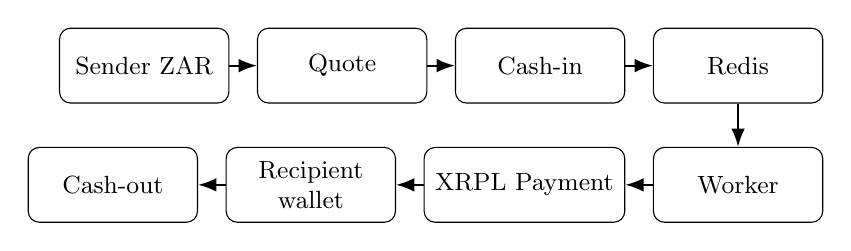
\begin{tikzpicture}[
  font=\small,
  box/.style={draw, rounded corners, align=center, inner sep=4pt, minimum height=0.95cm, minimum width=2.15cm},
  arr/.style={-{Latex}, thick}
]
\node[box] (zar) {Sender ZAR};
\node[box, right=0.35cm of zar] (q) {Quote};
\node[box, right=0.35cm of q] (ci) {Cash-in};
\node[box, right=0.35cm of ci] (rd) {Redis};
\node[box, below=0.55cm of rd] (w) {Worker};
\node[box, left=0.35cm of w] (pay) {XRPL Payment};
\node[box, left=0.35cm of pay] (wal) {Recipient\\wallet};
\node[box, left=0.35cm of wal] (co) {Cash-out};
\draw[arr] (zar) -- (q);
\draw[arr] (q) -- (ci);
\draw[arr] (ci) -- (rd);
\draw[arr] (rd) -- (w);
\draw[arr] (w) -- (pay);
\draw[arr] (pay) -- (wal);
\draw[arr] (wal) -- (co);
\end{tikzpicture}
\caption{Settlement path: confirmed rand in, queued Payment, custodial UCTUSD, simulated fiat out.}
\label{fig:flow}
\end{figure}

Wallet design is a hybrid of the brief's two options \citep{UCTBrief2026,UCTResources2026}. One \texttt{PlatformWallet} holds scarce IOU liquidity. Each recipient still receives a real custodial Testnet account, generated lazily on first settlement, so FR-style ``individually attributable Payment + hash'' is a genuine ledger transaction rather than a book entry that pretends to be one. Address and encrypted secret are committed \emph{before} TrustSet. If an address exists but the trust line is not yet established, the worker reuses the stored secret; it does not mint a second wallet.

XRP is the only asset an XRPL account holds natively; UCTUSD and RLUSD are issued tokens (IOUs). A holder can accept an IOU only after a TrustSet opens a trust line to the issuer, which reserves a little XRP (locked, not spent) \citep{UCTResources2026}. Rippling lets the same issued token move between holders of that issuer without an explicit hop back through the issuer: Default Ripple is normally on for the issuer and off for ordinary holders. We do not implement rippling ourselves; settlement is a direct treasury-to-recipient Payment after TrustSet.

\section{Cash-in, UCTUSD settlement, and cash-out}

\subsection{Cash-in}
\texttt{POST /remittances/\{id\}/cash-in} is allowed only on an unexpired, non-cancelled \texttt{quoted} remittance. The sender chooses \texttt{agent\_cash}, \texttt{bank\_transfer}, or \texttt{card}. Status becomes \texttt{cash\_in\_pending}. Admin \texttt{confirm-cash-in} sets \texttt{cash\_in\_confirmed} and calls \texttt{enqueue\_settlement}. No Payment is submitted at this step. The cash movement itself is simulated: there is no card acquirer, no agent till, and no bank confirmation webhook.

\subsection{UCTUSD settlement}
Enqueue inserts at most one \texttt{SettlementMessage} per remittance (unique constraint) and \texttt{XADD}s to stream \texttt{settlement\_messages}. The Redis Stream ID is stored on \texttt{stream\_entry\_id}. If the database row exists but the stream ID is missing or the entry is gone, a later enqueue \emph{republishes}---that covers ``DB commit succeeded, Redis \texttt{XADD} failed''. Redis is transport; the database row is source of truth.

The worker first reclaims its pending-entries list (\texttt{XREADGROUP} id \texttt{0}), then idle pending entries (\texttt{XAUTOCLAIM} on Redis~6.2+, else \texttt{XPENDING}+\texttt{XCLAIM}; local Memurai 5.0.14 has no \texttt{XAUTOCLAIM}), then new \texttt{>} entries. Entries are acknowledged only after the message is \texttt{completed} or \texttt{failed}. A crash mid-flight leaves the entry in the PEL for reclaim.

Before submitting a Payment, if \texttt{xrpl\_settlement\_tx\_hash} is already set, the worker marks completed and \textbf{does not pay or credit again}. On the success path the Payment memo carries the remittance id; the hash, recipient credit, \texttt{settled}, and \texttt{completed} are one database commit. Admin retry accepts \texttt{failed}, \texttt{processing}, and \texttt{pending} (reset to pending, republish). \texttt{completed} returns 409.

\subsection{Cash-out}
The recipient must have approved KYC to cash out but may hold UCTUSD without it. Spendable \texttt{RecipientWallet.balance} is debited atomically at request time (\texttt{UPDATE \ldots WHERE balance >= :amt}). \texttt{GET /wallet/me} reports \texttt{balance\_rlusd} and \texttt{spendable\_balance} as that spendable figure (the slot is currently UCTUSD; official RLUSD later via \texttt{.env} if funded). \texttt{on\_chain\_balance} is spendable plus cash-out amounts in \texttt{requested} or \texttt{approved} only; it excludes completed cash-outs. Fiat payout is still simulated, but complete submits a Payment of the reserved UCTUSD from the recipient custodial account to the official UCTUSD issuer (burn/redeem). After a request, spendable drops while on-chain stays higher by the reserved amount until complete, when the on-chain figure drops too. A failed cash-out refunds spendable.

\section{Database}
Runtime schema is Alembic, not \texttt{create\_all} alone. FastAPI lifespan runs \texttt{alembic upgrade head} then seeds default fees and limit tiers. Tests still use in-memory \texttt{create\_all}. Main tables:

\begin{itemize}
  \item \texttt{users} --- name, unique email and mobile, bcrypt \texttt{password\_hash}, role.
  \item \texttt{sessions} --- \texttt{token\_hash} (SHA-256 hex, unique), expiry, \texttt{revoked\_at}. No plaintext token column.
  \item \texttt{kyc\_applications} --- one row per user; identification number encrypted.
  \item \texttt{beneficiaries} --- payout profile; optional \texttt{linked\_user\_id}.
  \item \texttt{remittances} --- full lifecycle on one row: amounts, fees, status (including \texttt{cancelled}), \texttt{tracking\_ref}, \texttt{expires\_at}, cash-in fields, XRPL hash.
  \item \texttt{settlement\_messages} --- one per remittance; status; \texttt{stream\_entry\_id}; attempts; failure reason.
  \item \texttt{recipient\_wallets} --- custodial address, encrypted secret, trust-line flag, spendable \texttt{balance}. No \texttt{on\_chain\_balance} column; that figure is computed on read.
  \item \texttt{platform\_wallet} --- singleton treasury address and encrypted secret.
  \item \texttt{cash\_out\_requests} --- RLUSD amount, fiat, fee, payout, status, admin action stamps.
  \item \texttt{fee\_config}, \texttt{limit\_tiers} --- singleton fees; unverified/verified caps.
\end{itemize}

Encrypted columns are stored as \texttt{VARCHAR(500)} (Fernet ciphertext). Existing SQLite files created only with \texttt{create\_all} have no \texttt{alembic\_version} table and will fail upgrade; demo databases should start empty and migrate.

A remittance points at one sender and one beneficiary. A settlement message points at one remittance. A recipient wallet is 1:1 with a user. Cash-out requests belong to the recipient user, not to a remittance row: the recipient may cash out aggregated RLUSD, not a single inbound Payment. Platform wallet is a singleton.

\section{API overview}
The API is JSON over HTTP with Bearer sessions. FastAPI emits Swagger UI at \url{http://127.0.0.1:8000/docs} and the OpenAPI schema at \texttt{/openapi.json}. Route prefixes: auth, users, kyc, beneficiaries, remittances, limits, wallet, cash-outs, and admin (fees, limits, settlement, platform wallet). CORS defaults allow Vite on 5173 and 5174 (\texttt{localhost} and \texttt{127.0.0.1}), local React on 3000, and the API host on 8000, overridable with \texttt{CORS\_ORIGINS} as a JSON list. Credentials are allowed. The SPA stores the bearer token in \texttt{sessionStorage} and sends it as \texttt{Authorization: Bearer}.

Authz in short: customers act on their own resources; KYC-approved customers create quotes, beneficiaries, cash-in, and cash-outs; admins review KYC, confirm cash-in, run and retry settlement, action cash-outs, and edit fees and tiers. Tracking is visible to the sender, the linked recipient, or an admin (403 otherwise; 404 if the ref does not exist).

\section{Security}
Passwords are bcrypt via passlib and never stored in plaintext. Login returns a urlsafe bearer token once; the database stores only \texttt{SHA-256} of that token. Logout sets \texttt{revoked\_at}. Opaque sessions were chosen over JWT because this is a single FastAPI process: logout must actually revoke access, which a signed JWT cannot do without a server-side denylist that looks like the sessions table anyway.

Two Fernet keys are required: \texttt{KYC\_ENCRYPTION\_KEY} for the identification number, \texttt{XRPL\_KEY\_ENCRYPTION\_KEY} for platform and recipient XRPL secrets. A leak of one category does not decrypt the other. Keys live in environment variables, not in the database, not in API responses, not in application logs, and not in git (\texttt{.env} is local; \texttt{.env.example} has placeholders). XRPL secrets are decrypted only in the signing path. Bad ciphertext raises \texttt{RuntimeError} rather than returning empty values. Private keys are never printed by \texttt{setup\_platform\_wallet}. There is no custom application logger beyond uvicorn's access log (method/path/status, no bodies).

CORS is a demo convenience for the local Vite origin, not an authentication mechanism. Production would restrict origins, put keys in a secrets manager, rotate Fernet keys with a dual-decrypt window, and stop using SQLite as the vault for encrypted seeds.

\newpage
\section{Regulatory considerations}
This section is an understanding of the problem, not a legal opinion \citep{UCTBrief2026}. A Testnet IOU does not make the operator a licensed money transmitter, and it does not take the corridor outside FICA or SARB rules.

\paragraph{KYC and AML.}
South African accountable institutions under FICA must identify customers and understand source of funds before providing money-remittance services. Our mock KYC collects the brief's fields, encrypts the ID number, and gates sending and cash-out on admin approval. That is a teaching model of a control, not a CDD programme: we do not screen against sanctions lists, we do not verify documents against Home Affairs, and we do not file suspicious-transaction reports.

\paragraph{Transaction monitoring (not fully automated).}
A real remittance business is expected to monitor velocity, structuring, mule patterns, and corridor risk. We enforce daily and monthly ZAR caps and keep a full remittance and settlement audit trail, including XRPL hashes. We do \emph{not} ship an AML product: no rules engine, no alert queue, no SAR workflow. Operators would still need people and systems we have not built.

\paragraph{Custody of crypto assets.}
Recipient wallets are custodial: the platform generates Testnet keys, encrypts them, and signs on the customer's behalf. That is convenient and it is also a custody business. In production that would engage crypto-asset service-provider expectations (safekeeping, segregation, operational resilience) under the evolving South African CASP / FSCA framework. We store keys encrypted with a dedicated Fernet key; we do not offer self-custody withdrawal of the secret.

\paragraph{SARB and exchange control.}
Cross-border rand payments sit inside South African exchange-control and authorised-dealer arrangements. A stablecoin hop does not create a new legal corridor. Our cash-in is simulated, so we never actually take rand across the border. A live system would still need an authorised channel for the fiat legs and would still need to report what the SARB requires. RLUSD on Testnet is not a SARB-approved mechanism for discharging an exchange-control obligation.

\paragraph{Licensing.}
A commercial Western Union competitor in South Africa typically needs a FICA accountable-institution posture, Reserve Bank authorisation where the activity is a remittance or payment service, and---if offering crypto custody or exchange---the applicable FSCA crypto-asset authorisation. Agent cash-in/out may also engage payment-system and consumer-protection rules (clear fees, receipts, complaint handling). This coursework prototype is not licensed and must not be pointed at real customer funds or Mainnet credentials \citep{UCTBrief2026}.

Consumer protection and safeguarding follow from the same honesty: quoted fees should match charged fees (our quote locks the breakdown for 15 minutes); customer secrets should not leak (Section~11); and simulated balances must not be described as redeemable bank money. We do not hold client fiat in a trust account because we never collect real fiat. The web UI in Section~\ref{sec:ui} shows the locked fee breakdown, the \texttt{MG} tracking reference, and an academic contact block (course, group, campus, repository). That is coursework disclosure, not a licensed complaints desk.

\section{Assumptions and limitations}
Assumptions we adopted on purpose: one customer identity for send and receive; admins only via \texttt{scripts/create\_admin.py}; one KYC row with overwrite-on-resubmit until approved; beneficiary auto-match rather than invite-to-register; hybrid treasury plus per-recipient XRPL accounts; issuer address and currency code as \texttt{.env} so UCTUSD versus RLUSD is a config change \citep{UCTResources2026}; Redis Streams as the queue; SQLite for development; quote TTL of 900 seconds.

Remaining limitations of \emph{this} fork, not of the old sketch:
\begin{itemize}
  \item SQLite's single-writer model is not a production remittance ledger.
  \item Cash-in and fiat cash-out are simulated; complete still burns reserved UCTUSD on-chain by paying the issuer.
  \item Automated tests mock XRPL (faucet, TrustSet, Payment). Redis is real (DB~15).
  \item Redis is required at runtime and in pytest.
  \item Login latency is dominated by bcrypt (see Section~\ref{sec:perf}).
  \item No AML monitoring product, no sanctions screening, no production key-management service.
\end{itemize}

\section{Performance summary}
\label{sec:perf}
HTTP load was re-run on this fork on 7~September 2026 (50 concurrent synthetic users, 60~s, Windows, single-process uvicorn and SQLite). The tables and charts live in \texttt{PERFORMANCE\_TESTING.md} and \texttt{backend/perf/results/}. Five live Testnet Payments from 1~September 2026 remain the settlement sample---that path was not repeated against the demo treasury.

The 7~September mix delivered 2{,}218 requests, zero failures, about 37~req/s. Authenticated reads sat around 20--33~ms at the median; \texttt{POST /remittances} about 66~ms median. \texttt{POST /auth/login} remains the outlier (about 850~ms median) because bcrypt is deliberately expensive. Queue enqueue on this OneDrive-backed SQLite host measured about 23 messages/s (a 1~September Mac sample of the same Redis path was 517~msg/s). Five real Testnet Payments averaged about 12.4~s each---ledger close time, not application CPU. Relative bottlenecks---bcrypt on login, consensus on settlement---are unchanged in kind.

\newpage
\section{Web UI}
\label{sec:ui}
The marked web application is \texttt{frontend/}: Vite, React, TypeScript, and React Router. It calls the FastAPI JSON API with \texttt{VITE\_API\_URL} (default \url{http://127.0.0.1:8000}). The landing page is a marketing scroll (hero, quote explainer as \texttt{\#faq}, beneficiary/scan/methods, contact as \texttt{\#contact}, footer). Login, register, and the authenticated shells use a DASH-style grid-trail background. Landing motion is GSAP ScrollTrigger plus original Three.js objects---not third-party brand assets.

Table~\ref{tab:ui} is the shipped screen map. The quote screen shows send amount, locked transaction fee, net ZAR after that fee, FX margin, rate, and UCTUSD. Empty states are implemented, not planned: unverified senders see KYC pending, not a send form; expired quotes show expired and hide cash-in; a recipient without a Testnet account yet still sees a zero spendable wallet row; settlement failure shows the worker reason (for example \texttt{tecPATH\_DRY}) rather than a dummy hash.

\begin{table}[H]
\centering
\caption{Shipped screens mapped to routes and endpoints.}
\label{tab:ui}
\footnotesize
\begin{tabular}{@{}p{0.20\textwidth}p{0.22\textwidth}p{0.50\textwidth}@{}}
\toprule
\textbf{Screen} & \textbf{Route} & \textbf{Endpoints} \\
\midrule
Landing / FAQ / Contact &
\texttt{/}, \texttt{\#faq}, \texttt{\#contact} &
static; Contact states course, group, campus, GitHub \\
Register / login &
\texttt{/register}, \texttt{/login} &
\texttt{POST /auth/register}, \texttt{/login}, \texttt{/logout} \\
Sender home &
\texttt{/app} &
\texttt{GET /users/me}, \texttt{/kyc/me/status}, \texttt{/limits/me} \\
Profile &
\texttt{/app/profile} &
\texttt{GET}/\texttt{PATCH /users/me} \\
KYC form &
\texttt{/app/kyc} &
\texttt{POST /kyc}, \texttt{GET /kyc/me} \\
Beneficiaries &
\texttt{/app/beneficiaries} &
\texttt{GET}/\texttt{POST /beneficiaries} \\
New quote / quote &
\texttt{/app/send}, \texttt{/app/send/\{id\}} &
\texttt{POST /remittances}, \texttt{\ldots/cancel}, \texttt{\ldots/cash-in} \\
History / track &
\texttt{/app/history}, \texttt{/app/track/\{ref\}} &
\texttt{GET /remittances/me}, \texttt{/remittances/track/\{ref\}} \\
Recipient wallet &
\texttt{/app/wallet} &
\texttt{GET /wallet/me} \\
Cash-out &
\texttt{/app/cash-out} &
\texttt{POST /cash-outs}, \texttt{GET /cash-outs/me} \\
Admin KYC &
\texttt{/admin/kyc} &
\texttt{GET /kyc}, \texttt{POST \ldots/approve\textbar reject} \\
Admin cash-in &
\texttt{/admin/cash-in} &
\texttt{GET /remittances}, \texttt{POST \ldots/confirm-cash-in} \\
Admin settlement &
\texttt{/admin/settlement} &
\texttt{GET /admin/settlement}, \texttt{POST \ldots/run}, \texttt{\ldots/\{id\}/retry} \\
Admin cash-out &
\texttt{/admin/cash-out} &
\texttt{GET /cash-outs}, \texttt{POST \ldots/approve\textbar complete\textbar fail} \\
Admin config &
\texttt{/admin/config} &
\texttt{GET}/\texttt{PUT /admin/fee-config}, \texttt{/admin/limit-tiers} \\
Platform wallet &
\texttt{/admin/platform-wallet} &
\texttt{GET /admin/platform-wallet}; TrustLine helper \\
\bottomrule
\end{tabular}
\end{table}

Admins are created with \texttt{scripts/create\_admin.py}, never via public register. The examiner demo is the UI at \url{http://127.0.0.1:5173/} (or 5174) against the API on 8000: register or sign in, KYC, beneficiary, quote, cash-in, admin confirm, settlement run or retry, track, then recipient wallet and optional cash-out. Swagger at \texttt{/docs} remains a developer tool, not the marked product.

\bibliographystyle{apalike}
\bibliography{../refs}

\end{document}
